%% ----------------------------------------------------------------
%% Testing.tex
%% ---------------------------------------------------------------- 

\chapter{Testing} \label{Chapter: Testing}


\chapterpreamble{Software testing is necessary on projects of all sizes, especially on large projects such as this. To ensure quality throughout the project each part of the framework has been throughly tested. This chapter details different testing methodologies along with the results of the tests. }

\section{Introduction}

Talk about testing and how we will perform it.

\section{Tools}

\subsection{karma}

Karma is a test runner.

\subsection{Jasmine}

Jasmine is a testing framework for JavaScript.


Reference different plugins

Motivation for this.

{for section in sections: describe section}

\section{Videogular Questions Example} 
\label{Section:Videogular Questions Example}

The Videogular Questions Example site was written as testing and documentation for how Videogular Questions and Videogular Cuepoints could be used. 

\subsection{Videogular Questions}
\label{Subsection:Videogular Questions in example}

There are several tests written for the vgQuestions plugin. These use Jasmine, and can be run in an automated way using karma.

These tests exercise the web worker component of the vgQuestions plugin over the message passing interface. A script is used, which contains messages to send, and expected responses. A test passes if the script runs as expected with no missing or extra messages.

The examples created in the (videogular-questions-example) repository, use individual or collections of features. These were used in the development of these features, and in the demonstration of these features to the customer.  These examples complement the Jasmine tests, as they exercise the display elements of the plugin.

Client had reservations about UX testing due to toolkit style nature of the project. Shameem did so, results were interesting (possibly useful) \todo{Flesh out}

\subsection{Videogular Cuepoints}
\label{Subsection:Videogular Cuepoints in example}
\gls{Videogular} Cuepoints was integrated into the example site, and configured to mark the times at which pop-ups were displayed. The issue where marks could only be displayed once the video began to play (as described in \autoref{Subsection:vgCuepoints}) was the only problem encountered.

\subsection{Example Results Server}
\label{Subsection:Example Results Server in example}
For the example results server we had a small set of functions to test with a small number of possible inputs and a well defined set of responses. This is a therefore well suited to individual unit tests.

Flask\footnote{\url{http://flask.pocoo.org/}} is a python web application framework that allows you to create web applications with simple routing patterns in Python.

The flask library had a test client and recommended test skeleton\footnote{\url{http://flask.pocoo.org/docs/0.10/testing/}} which we made use of to run the unit tests. This used the unittest standard python library which meant it was easy to test with but also allowed calling of methods by simulating HTTP requests.

These tests are recommended to be run before committing new code to the repository and formed one part of the quality assurance testing. Any tests that failed were reviewed before committing and fixed if they were at fault. No code should have been committed to master branches that caused tests to fail. All code on the master branch was expected to pass these tests on checkout.

We split the testing into 6 areas to test the main components of the application.

\subsubsection{Cross-Origin Resource Sharing tests}

One of the main requirements by the customer was that these units should be able to be accessed via REST calls (see \cref{Req:Server architecture}). In addition the requirement stated that there should be no reliance that these servers are on the same host. To ensure that these REST calls will not fail we need to implement cross origin resource sharing headers as discussed in \autoref{Section:Modular Approach}.

This checks to ensure that the CORS header is correctly sent in the HTTP reply. If this is not set the web browser will likely reject the loading of the page and the application will fail.

In addition, it ensures that the response is the one expected and not an error state to ensure that the web application is also sending the correct content.

\subsubsection{Routing tests}

The routing tests are to ensure that the application correctly starts and is accessible.

If this fails to load up the testing URL which returns "Hello World!" then it is unlikely to be able to perform some of the more complex functions.

\subsubsection{Database Setup tests}

Before the application can be used it needs have its database set up. This is performed by accessing `/setup'. This set of unit tests test setting up a database and ensure that if this URL is visited twice, it successfully detects that the database is already set up and does not recreate it. 

This is important to ensure that the database is set up correctly and that when setup is visited again data in the database is not lost.

\subsection{Voting tests}

These tests try a number of different ways to vote by sending a number of different formats of invalid and valid data to check if the application correctly deals with the data. All return codes and responses are checked to ensure no invalid vote is accepted or valid one rejected.

\subsubsection{Getting results tests}

A number of valid votes are constructed and then sent into the system. Then these are attempted to be retrieved. The returned values are checked to ensure that they have not been corrupted. This submits one and multiple votes to ensure that all votes are correctly collated and returned.

If the ability to vote does not work then this will fail as it relies on being able to put votes into the system.

\subsubsection{Load testing}

For load testing we have used Locust\footnote{\url{http://locust.io/}} which spawns a number of testing clients and executes a defined pattern of site usage.

We chose three patterns to test the example results server:

\begin{itemize}
\item Visiting the root page - This is to determine that the webserver is still responding to basic HTTP requests
\item Voting - This is to test that the voting functionality is still accessible
\item Requesting data - This is to test that the server is still able to return data
\end{itemize}

These three URL's were visited repeatedly by the user clients over a period of time.

\begin{table}
\caption{Time taken for each request to complete in milliseconds while stress testing the example results server}
\begin{tabular}{l c  c c c c c c c c }
\hline 
& & \multicolumn{8}{c}{Percentile} \\
Name & Requests & 50\% & 75\% & 80\% & 90\% & 95\% & 98\% & 99\% & 100\% \\ 
\hline 
GET / & 535 & 5 & 50 & 67 & 110 & 170 & 240 & 360 & 601 \\ 
\hline 
GET /results/*/* & 1599 & 6 & 26 & 46 & 100 & 136 & 233 & 326 & 326 \\ 
\hline 
POST /vote & 1129 & 120 & 150 & 170 & 210 & 250 & 360 & 460 & 638 \\ 
\hline 
Total / Average & 3263 & 32 & 110 & 120 & 160 & 210 & 270 & 400 & 638 \\ 
\hline 
\end{tabular}
\label{Table:stress_testing_results_server}
\end{table}

\autoref{Table:stress_testing_results_server} shows the time taken for a response to be handled and returned.

Here you can see that the time taken for result requests takes less than 6 milliseconds 50\% of the time and all requests were dealt with in at most 326 milliseconds. The voting REST point takes slightly longer as it needs to store data to the sqlite database but still took at max 638 milliseconds. All these tests were performed when 50 Locust users were using the website continuously and therefore we feel the performance wills scale. This is because one user will only ever make one vote and one results request per poll and this tested for 50 users continuously making these requests.

Although this is only an example this ties in with requirement \todo{reference requirement} that the results server should perform normally when a lecture room full of people is using it. The testing shows that the application is able to cope with 50 people continuously voting and therefore should be able to cope with a much less strenuous 300 people casting votes over a period of a couple minutes.

There is also scope to move the backend database to something that is purely in memory to further increase the speed, as the major factor will be writing the data back to the hard disk.

\section{Example Analytics}

\subsection{Back End - Example Analytics Server}
\label{Subsection:Analytics server in example}
Testing of sending events

Load testing

\subsection{Front End}
\subsubsection{Videogular Heatmaps}
\label{Subsubsection:Videogular Heatmaps in example}
%Heatmap, user stories, run through

One of the analytics used in the example site is the \gls{Videogular} Heatmap. When running an instance of \gls{Videogular} Questions Example this could be used to dynamically update the heat map in the example analytics page (see \autoref{Figure: Heat map display}).

\begin{figure}[h]
	\centering 
		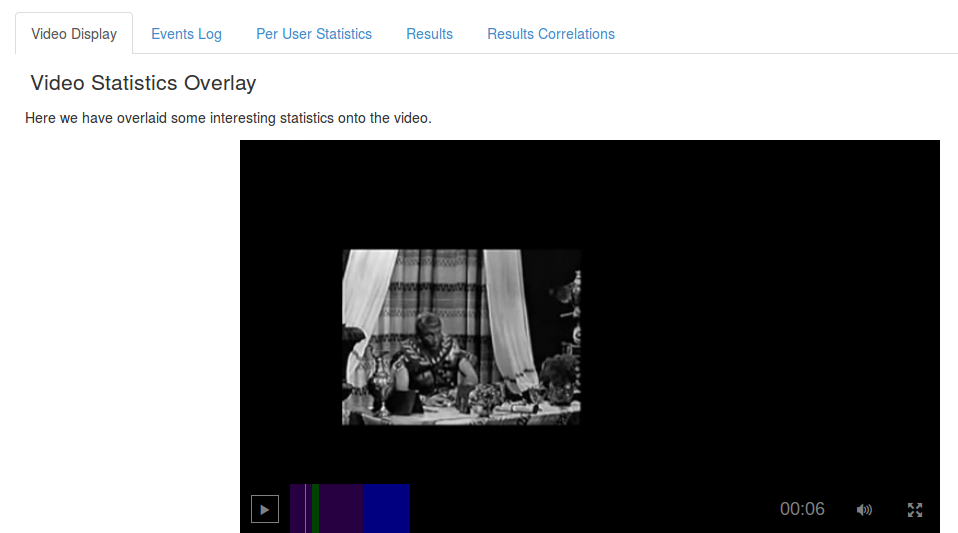
\includegraphics[scale=0.4]{../figures/heatmapDisplay.png} 		
	\caption{\label{Figure: Heat map display} The heat map has dynamically updated} 	
\end{figure}

The added feature of displaying the frequencies was also tested. These displayed well and matched the frequencies represented by the colours used. A screen reader could still access the data as it was declared in hidden text.

\section{Authoring Tool}

List of objectives

Deliverable report had a basic list of actions to "test"

\subsection{Accessibility}
The authoring tool was found to be generally accessible conforming to most of the WCAG 2.0 standards. The areas that were lacking were providing textual alternatives and error checking.

There were no alternatives provided for the video. However as this would be used with Synote transcripts could be used from there. In future, support for extra accessibility features such as transcripts, captions or signed versions could be included in the authoring tool.

In creating the questions there is no help provided for error checking. This is because it was decided not to narrow the options available to the users. In the occurrences where errors are identified these are generally highlighted by surrounding the component with a red border. More information on how the system would be used would be required in order to create helpful error messages.

\todo{Chrome's lack of multiple select}

Another issue found was in the use of the \texttt{\textless select\textgreater} element as the colour of highlighted options is not editable in the \gls{CSS}. To solve this issue the elements would all need rewriting to take a completely different structure to allow the \gls{CSS} to modify the colours used.

Accessibility in the authoring tool was good but there are improvements that could be made in future including adding support for accessibility features such as subtitles, providing error correction support and rewriting the \texttt{\textless select\textgreater} elements to allow editing of colours.


\section{Conclusion}

Comment on the conclusions of the testing.

